	\section{Potenciação}

    \noindent
	\textbf{Definição:} Sejam $a$ um número real e $n$ um número natural, tal que $ n \geq 2 $. Chama-se potência de base $a$ e expoente $n$ o número $n^a$, em que 
 
	\begin{tcolorbox}[colback=white,colframe=minha_cor,coltitle=black,title=Definição] 
        \[
        a^n = \underbrace{a \times a \times \cdots \times
			a}_{n \; vezes} \quad a \in\mathbb{R}, n \in\mathbb{N}, \geq 2.
        \]
        \end{tcolorbox}
	
	Dessa definição decorre que:
	\begin{equation}
		a^2 = a \cdot a, \;\; a^3 = a \cdot a \cdot a, \;\; a^4 = a \cdot a \cdot a \cdot a, \;\; etc.
		\nonumber
	\end{equation}

    \noindent
	\textbf{Definições Especiais}
	\begin{itemize}
		\item Para $n = 0$ e $a \neq 0$, $a^0 = 1$;
		\item Para $n = 1$, $a^1 = a$;
        \item Note a condição de existência $a \neq 0$, pois $0^0$ é indeterminado.
	\end{itemize}

        \begin{texample}
        \centering
        \tcbhighmath{2^4 = 2 \cdot 2 \cdot 2 \cdot 2 = 16}
        \tcbhighmath{\left(\dfrac{2}{3}\right)^3 = \dfrac{2}{3} \cdot \dfrac{2}{3} \cdot \df{2}{3} = \df{8}{27}}
        \end{texample}
 
	Quando o número base é negativo, o resultado será positivo para expoente par e negativo para expoente ímpar.Veja alguns exemplos:

        \begin{texample}
        \centering
        \tcbhighmath{(-2)^3 = (-2) \cdot (-2) \cdot (-2) = -8}
        \tcbhighmath{(-2)^4 = (-2) \cdot (-2) \cdot (-2) \cdot (-2) = 16}
        \tcbhighmath{\left(-\dfrac{2}{3}\right)^3 = \left(-\dfrac{2}{3}\right) \cdot \left(-\dfrac{2}{3}\right) \cdot \left(-\df{2}{3}\right) = -\df{8}{27}}
        \tcbhighmath{\left(-\dfrac{2}{3}\right)^4 = \left(-\dfrac{2}{3}\right) \cdot \left(-\dfrac{2}{3}\right) \cdot \left(-\df{2}{3}\right) \cdot \left(-\df{2}{3}\right)= -\df{16}{81}}
        \end{texample}
	
	\subsection{Propriedades}
	
	Sejam $a$ um número real e $m$ e $n$ números naturais.
	\begin{itemize}
		\item Multiplicação de potência de mesma base
		\begin{center}
			$(a)^m \cdot (a)^n = a^{m+n}$
		\end{center}
		\item Multiplicação de potência de bases diferentes e mesmo expoente
		\begin{center}
			$(a)^n \cdot (b)^n = (ab)^n$
		\end{center}
		\item Divisão de potências de mesma base
		\begin{center}
			$\dfrac{(a)^m}{(a)^n} = a^{m-n} ,\;\; a \neq 0$
		\end{center}
		\item Divisão de potências de bases diferentes e mesmo expoente
		\begin{center}
			$\dfrac{(a)^n}{(b)^n} = \left( \dfrac{a}{b} \right) ^{n} ,\;\; b \neq 0$
		\end{center}
		\item Potência de potência
		\begin{center}
			$ (a^m)^n = a^{mn}$
		\end{center}
	\end{itemize}    
	
	\subsection{Consequências}
	\begin{itemize}
		\item Potência de expoente negativo
		\begin{center}
			$ a^{-n} = \dfrac{1}{a^n}, \;\; a \neq 0$
		\end{center}
		pois, 
		\begin{center}   
			$a^{-n} = a^{0-n} = \dfrac{a^0}{a^n} = \dfrac{1}{a^n}$ 
		\end{center}
	\end{itemize}   
	
	     
    \begin{texample}
        \centering
        \tcbhighmath{2^{-3} = \dfrac{1}{2^3} = \dfrac{1}{8}}
        \tcbhighmath{2^{-4} = \dfrac{1}{2^4} = \dfrac{1}{16}}
        \tcbhighmath{\left(\dfrac{2}{3}\right)^{-2} = \left(\dfrac{3}{2}\right)^2 = \dfrac{9}{4}}
    \end{texample}

	\section{Radiciação}

    \noindent
	\textbf{Definição:} Dados um número real não negativo $a$ e um número natural $n$, $n \geq 1$, chama-se raiz enésima aritmética de um número $a$ o número real $b$ e não negativo tal que $b^n = a$.
	
	A radiciação é a operação inversa da potenciação. De modo geral, tem-se:
	\begin{tcolorbox}[colback=white,colframe=minha_cor,coltitle=black,title=Definição] 
        \begin{center}
            \begin{minipage}{0.8\textwidth}
            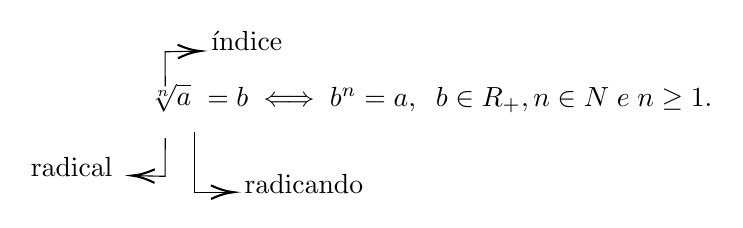
\begin{tikzpicture}[x=0.75pt,y=0.75pt,yscale=-1,xscale=1]
            \draw    (87,162) -- (87,191) -- (104,191) ;
            \draw [shift={(106,191)}, rotate = 180] [color={rgb, 255:red, 0; green, 0; blue, 0 }  ][line width=0.75]    (10.93,-3.29) .. controls (6.95,-1.4) and (3.31,-0.3) .. (0,0) .. controls (3.31,0.3) and (6.95,1.4) .. (10.93,3.29)   ;
            \draw    (73,165) -- (72.97,183.35) -- (59,183.04) ;
            \draw [shift={(57,183)}, rotate = 1.26] [color={rgb, 255:red, 0; green, 0; blue, 0 }  ][line width=0.75]    (10.93,-3.29) .. controls (6.95,-1.4) and (3.31,-0.3) .. (0,0) .. controls (3.31,0.3) and (6.95,1.4) .. (10.93,3.29)   ;
            \draw    (73,140) -- (72.97,123.35) -- (88,123.04) ;
            \draw [shift={(90,123)}, rotate = 178.81] [color={rgb, 255:red, 0; green, 0; blue, 0 }  ][line width=0.75]    (10.93,-3.29) .. controls (6.95,-1.4) and (3.31,-0.3) .. (0,0) .. controls (3.31,0.3) and (6.95,1.4) .. (10.93,3.29)   ;
            \draw (64,137.4) node [anchor=north west][inner sep=0.75pt]    {$\sqrt[n]{a}$};
            \draw (94,112) node [anchor=north west][inner sep=0.75pt]   [align=left] {índice};
            \draw (110,181) node [anchor=north west][inner sep=0.75pt]   [align=left] {radicando};
            \draw (7,173) node [anchor=north west][inner sep=0.75pt]   [align=left] {radical};
            \draw (92,139) node [anchor=north west][inner sep=0.75pt]    {$ = b \iff  b^n = a, \;\; b \in\mathbb{{R_+}}, n \in\mathbb{N} \;e \;n \geq 1.$};
            \end{tikzpicture}
            \end{minipage}
        \end{center}
    \end{tcolorbox}

    \noindent   
	isto é, o resultado $b$ da raiz enésima de um número $a$ corresponde à expressão deste número $b$ elevado a $n$ com resultado $a$.
    
	Todo radical pode ser escrito na forma de uma potência fracionária
	
	\[
		\sqrt[n]{a} = a^{\frac{1}{n}}
	\]
	
	Note que para $n = 2$, a notação reduz-se a
	
	\[
		\sqrt{a}
	\]
	
	Isto é, quando o índice da raiz é igual a 2, é possível omiti-lo. Além disso, note que
	
	\[
		\sqrt{x^2} = | x |
	\]
	
	Usando a definição:

        \begin{texample}
        \centering
        \tcbhighmath{\sqrt[2]{9} = 3 \iff 3^2 = 9}
        \tcbhighmath{\sqrt[3]{8} = 2 \iff 2^3 = 8}
        \tcbhighmath{\sqrt[3]{0} = 0 \iff 0^3 = 0}
        \tcbhighmath{\sqrt[4]{625} = 5 \iff 5^4 = 625}
        \end{texample}
	
	Usando expoente fracionário e propriedades de potência
	\begin{texample}
        \centering
        \tcbhighmath{\sqrt[2]{9} = 9^{\frac{1}{2}} = (3^2)^{\frac{1}{2}} = 3^{2 \cdot \frac{1}{2}}  = 3}
        \tcbhighmath{\sqrt[3]{8}= (2^3)^{\frac{1}{3}} = 2^{3 \cdot \frac{1}{3}}  = 2}
        \tcbhighmath{\sqrt[3]{0} = 0^{\frac{1}{3}} = 0}
        \tcbhighmath{\sqrt[4]{625} = (5^4)^{\frac{1}{4}} = 5^{4 \cdot \frac{1}{4}}  = 5}
        \end{texample}
	
	\subsection{Propriedades}
	\begin{itemize}
		\item Potência de uma raiz de índice e expoente iguais
		\begin{equation}
			(\sqrt[n]{a}) ^ {n} = \left(a^{\frac{1}{n}}\right)^n = a^{\frac{n}{n}} = a
			\nonumber    
		\end{equation}
		\item Potência de uma raiz de índice e expoente diferentes
		\begin{equation}
			\left(\sqrt[n]{a}\right)^m = \left(a^{\frac{1}{n}}\right)^m = a^{\frac{m}{n}} = \sqrt[n]{a^m}
			\nonumber    
		\end{equation}
		\item Raiz de uma raiz
		\begin{equation}
			\sqrt[m]{\sqrt[n]{a}} = \left(a^{\frac{1}{n}}\right)^{\frac{1}{m}} = a^{\frac{1}{nm}} = \sqrt[nm]{a}
			\nonumber    
		\end{equation}
		\item Multiplicação de raízes com mesmo índice
		\begin{equation}
			\sqrt[n]{a} \cdot \sqrt[n]{b} \cdot \sqrt[n]{c} = \sqrt[n]{abc}
			\nonumber    
		\end{equation}
		\item Divisão de raízes com mesmo índice
		\begin{equation}
			\dfrac{\sqrt[n]{a}}{\sqrt[n]{b}} = \sqrt[n]{\df{a}{b}}
			\nonumber    
		\end{equation}
	\end{itemize}
	
	\section{Exercícios}
 
    \begin{enumerate}
	 %  \item Fatore e simplifique as expressões, usando propriedades de potências e radicais
	%\begin{itemize}
	%	\item $\dfrac{\sqrt[6]{a^2 b^3}}{(a^2)^3 \sqrt[2]{b^7}}$
	%	\item $\dfrac{\sqrt{27} \cdot \sqrt[3]{24}}{54 \cdot 14}$
	%\end{itemize}

		\item Obtenha o valor da expressão $\dfrac{3^{x+2} + 3^{x+1}}{3^{x+1}}$
		
		\item A fração $\dfrac{2^{98}+4^{50}-8^{34}}{2^{99}-32^{20}+2^{101}}$ é equivalente a 
		\begin{enumerate}
			\item $-1$
			\item $\dfrac{-11}{6}$
			\item $2$
			\item $\dfrac{-5}{2}$
			\item $\dfrac{7}{4}$
		\end{enumerate}
		
		\item Simplifique as expressões abaixo:
		\begin{enumerate}
			\item $\dfrac{2^3}{2^{-2}}$
			\item $-\sqrt[3]{-8}$
			\item $(3^5)(9^2)$
		\end{enumerate}
		
		\item Marque as sentença como verdadeiras ou falsas.
		\begin{enumerate}
			\item \text{[ \;\;]} $x^{-4} > x^{-3}$
			\item \text{[ \;\;]} $y^{-b} = \dfrac{1}{y^{ab}}$
			\item \text{[ \;\;]} $\sqrt{x^4} = x^2$
			\item \text{[ \;\;]} $\sqrt{16} = \pm 2$
		\end{enumerate}
		
		\item Calcule o valor da expressão $\dfrac{\sqrt[3]{3^n-9^n}}{\sqrt[3]{\sqrt[4]{9^n} \sqrt{3^n}}}$
		
		\item Simplifique as expressões abaixo 
		\begin{enumerate}
			\item $\sqrt{8} + \sqrt{18}$
			\item $\sqrt{x} \sqrt{32 y^{4} x}$
			\item $\dfrac{x}{\sqrt{9}}(\sqrt[3]{-8} + 5 \sqrt[5]{-32})$
			\item $ (a^{-1})^2 + (b^2)^{-1} +2(ab)^{-1}$
		\end{enumerate}
	\end{enumerate}
	
	
	\section{Respostas dos exercícios}
 
	\begin{enumerate}
		\item $4$
		\item $\dfrac{-11}{6}$    
		\item Simplifique as expressões abaixo:
		\begin{enumerate}
			\item $2^5$
			\item $2$
			\item $3^9$
		\end{enumerate}
		
		\item Marque as sentença como verdadeiras ou falsas.
		\begin{enumerate}
			\item \text{[ F ]}
			\item \text{[ V ]}
			\item \text{[ V ]}
			\item \text{[ F ]}
		\end{enumerate}
		
		\item  $\sqrt[3]{1-3^n}$
		
		\item Simplifique as expressões abaixo 
		\begin{enumerate}
			\item $5\sqrt{2}$
			\item $4xy^2\sqrt{2}$
			\item $-4x$
			\item $ \left(\dfrac{a+b}{ab}\right)^{2}$
		\end{enumerate}
	\end{enumerate}

 